\documentclass[a4paper, 12pt]{article}
\usepackage[utf8]{inputenc}
%\usepackage[T1]{fontenc}
\usepackage[serbian]{babel}
\usepackage{amsmath}
\usepackage[margin = 2cm]{geometry}
\usepackage{graphicx}
\usepackage{nopageno}
\usepackage{blindtext}
\usepackage{tabularx}
\usepackage{multirow}
\usepackage{subcaption}
\usepackage{tikz}

\newcolumntype{R}{>{\raggedleft\arraybackslash}X}
\newcolumntype{C}{>{\centering\arraybackslash}X}

\graphicspath{ {./img/} }

\pagestyle{empty}
\newcommand{\btmline}{
\vfill
\rule{0.9\textwidth}{0.4mm}
\begin{center}
13E043RE - Računarska elektronika
\end{center}}

\newcommand{\Huff}{\emph{Huffman}}

\title{
\Large{Univerzitet u Beogradu - Elektrotehnički fakultet}\\
\vspace{0.5cm}
\large{Katedra za elektroniku}\\
\vspace{1.2cm}
\begin{figure}[h!]
\centering

\includegraphics[scale=1.2]{logo}
\end{figure}
\vspace{3cm}
\Huge{\textbf{\textit{Huffman Coding}}} \\
\vspace{0.5cm}
\Large{\textbf{Implementacija u MASM asemblerskom jeziku}}\\
\vspace{2cm}
\Large{13E043RE - Računarska elektronika}\\
\vfill
}
\author{Radomir Vranjevac 2017/0103\\Dušan Ilić 2017/0070}
\date{}


\renewcommand{\arraystretch}{1}
%==========================================================================
\begin{document}
%==========================TITLE===========================================
\maketitle
\newpage
%==========================================================================

\section*{Zadatak}

Potrebno je napisati program u \textbf{MASM} jeziku koji vrši \textit{Huffman}-ovo kodovanje simbola. Ovo
kodovanje zasnovano je na verovatnoći pojavljivanja simbola gde se simboli sa najvećom verovatnoćom
pojavljivanja koduju sa kodnom rečju najmanje dužine.

Nakon pokretanja programa od korisnika se traži da unese naziv tekstualne datoteke nad kojom želi
da primeni mehanizam \textit{Huffman}-ovog kodovanja. Kao rezultat kodovanja na konzoli se ispisuje
učestanost pojavljivanja pojedinih simbola kao i kodne reči koje su dodeljene pojedinom simbolu.

\btmline\newpage
%==========================================================================

\section*{Uvod}

\textit{Huffman}-ovo kodovanje predstavlja algoritam za kodovanje simbola, gde dužina koda svakog simbola zavisi
od učestanosti ponavljanja datog simbola u određenom tekstu, odnosno tekstualnoj datoteci. Cilj je da se kodovanjem
smanji potreban memorijski prostor za čuvanje sadržaja nekog fajla.

\textit{Huffman}-ovo kodovanje spada u \textit{prefix} kodove, odnosno zadovoljava pravilo da nijedan k\^ od nije prefiks nekog drugog koda
(kodovi u kojima je svaki simbol predstavljen istim brojem bita automatski zadovoljavaju pravilo prefiksa).
Ovo predstavlja dobru osobinu jer znatno olakšava dekodovanje.

U daljem tekstu će detaljno biti objašnjen postupak kodovanja.

\subsection*{Struktura projekta}

Prilikom izrade projekta, projekat je podeljen na logičke celine. Ceo projekat se sastoji iz sledećih delova i fajlova:

\begin{enumerate}
\item \textbf{Konfiguracija} - sadrži fajl u kojem se nalaze definicije konstanti i parametara korišćenih u projektu, poput maksimalne dužine niza itd.
	\begin{itemize}
	\item \verb|configuration.inc|
	\end{itemize}
	\item \textbf{Složene strukture} - sadrži fajl u kojem se nalaze definicije složenih struktura podataka koje su korišćene prilikom izrade projekta.
	\begin{itemize}
	\item \verb|structures.inc|
	\end{itemize}
\item \textbf{Rad sa tekstualnom datotekom} - sadrži fajlove za deklaracije i definicije procedura korišćenih za obradu sadržaja tekstualne datoteke.
	\begin{itemize}
	\item \verb|file_process.inc|
	\item \verb|file_process.asm|
	\end{itemize}
\item \textbf{Formiranje \textit{Huffman}-ovog stabla i rad sa njim} - sadrži deklaracije i definicije procedura korišćenih za rad sa \textit{Huffman}-ovim stablom.
	\begin{itemize}
	\item \verb|huffman_tree.inc|
	\item \verb|huffman_tree.asm|
	\end{itemize}
\item \textbf{Glavni program} - sadrži glavni program koji koristi sve pomoćne procedure definisane u ostalim fajlovima.
	\begin{itemize}
	\item \verb|main.asm|
	\end{itemize}
\end{enumerate}

\btmline\newpage
%==========================================================================

\subsubsection*{\textit{Include} fajlovi}
Svaki \verb|.inc| fajl zaštićen je od višestrukog uključivanja u projekat definisanjem makroa, čije se postojanje proverava prilikom uključivanja u projekat.
Primer koda koji ovo obezbeđuje prikazan je u nastavku.

\begin{verbatim}
ifndef _FILENAME_INC_
_FILENAME_INC_ = 0

	; content goes here
	
endif
\end{verbatim}

\subsubsection*{Strukture podataka}
Grafički prikaz struktura koje su korišćene prikazan je na slici \ref{struct}. 

\begin{figure}[h!]
\centering
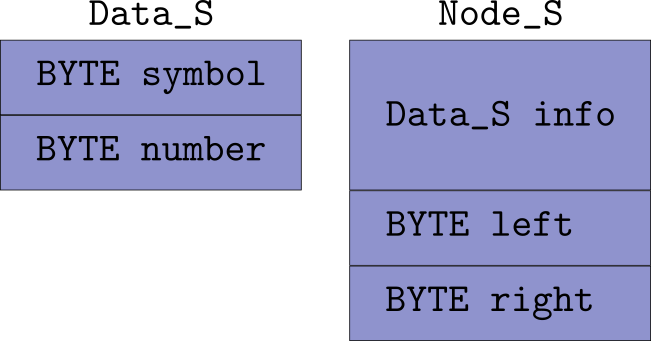
\includegraphics[width=.5\textwidth]{structures}
\caption{Strukture podataka}
\label{struct}
\end{figure}

Polje \verb|symbol| strukture \verb|Data_S| sadrži karakter, a polje \verb|number| sadrži njegov broj ponavljanja.
Struktura \verb|Node_S| predstavlja čvor u \textit{Huffman}-ovom stablu . Polja \verb|left| i \verb|right| koriste se 
za određivanje deteta datog čvora. 

\Huff-ovo stablo se čuva u obliku dvostruko ulančanog niza, gde polja \verb|left| i \verb|right| sadrže indekse čvorova oba deteta u istom nizu.

\btmline\newpage
%==========================================================================

\section*{Rad sa datotekom}



\btmline\newpage
%==========================================================================
\section*{Formiranje stabla}
Nakon sortiranja struktura \verb|Data_S| u nerastućem poretku po broju pojavljivanja karaktera, potrebno je formirati \emph{Huffman}-ovo stablo. \\
Osnovni princip iza \Huff-ovog algoritma je združivanje dva čvora sa najmanjim brojem pojavljivanja. Ti čvorovi u prvoj iteraciji predstavljaju listove stabla, odnosno dva najređe korišćena karaktera u ulaznoj datoteci. Od njih se pravi novi čvor, sa ekvivalentnim brojem pojavljivanja jednakim zbiru pojavljivanja dva karaktera od kojih je sačinjen.

Primera radi, biće pokazan algoritam formiranja stabla na ulaznim podacima sledećeg sadržaja (navedeni su karakter i broj njegovog pojavljivanja):
\begin{table}[ht]
	\centering
	\begin{tabular}{| c ||  c  c  c  c  c  c  c  c |}
		\hline
		$c$ & z & k & m & c & u & d & l & e \\ \hline
		$n$ & 2 & 7 & 24 & 32 & 37 & 42 & 42 & 120 \\ \hline
	\end{tabular}
\end{table}

Počinje se združivanjem karaktera \verb|z| i \verb|k| koji zajedno čine čvor stabla (tipa \verb|Node_S|) koji nema reprezentujući karakter, ekvivalentni broj pojavljivanja mu je $9$, i sadrži reference na čvorove ispod sebe (decu). 

Takav čvor (bez karaktera) se stavlja u privremeni niz, gde čeka da bude združen sa drugim takvim čvorom, ili sa novim karakterom. U oba slučaja, iskorišćeni čvor se briše; a novodobijeni čvor se dodaje u privremeni niz. \\
Nakon navedenog združivanja, dva čvora sa najmanjim brojem pojavljivanja su:
\begin{itemize}
	\item Novodobijeni čvor sa 9 pojavljivanja
	\item Karakter \verb|m| sa 24 pojavljivanja
\end{itemize}
Algoritam se zatim ponavlja u krug: \\
Združivanjem ta dva čvora dobija se novi čvor kome je ekvivalentni broj pojavljivanja jednak $33$, \ldots

Pogodno je primetiti da su dva najređa čvora uvek jedna od sledećih mogućnosti:
\begin{enumerate}
	\item \textbf{Dva nova karaktera} ukoliko su brojevi pojavljivanja sledeća dva neiskorišćena karaktera manja od broja pojavljivanja svakog čvora u privremenom nizu
	\item \textbf{Dva čvora iz privremenog niza} ukoliko su brojevi pojavljivanja čvorova u privremenom nizu (posmatrajući najmanja dva) manji od broja pojavljivanja najređeg neiskorišćenog karaktera
	\item \textbf{Jedan novi karakter i jedan čvor iz privremenog niza} u ostalim slučajevima
\end{enumerate}

U cilju određivanja koji elementi će biti združeni, dovoljno je izvršiti do dva poređenja čvorova, i poređenja dužina privremenog niza sa 2, i broja preostalih elemenata ulaznog niza sa 2 (očigledno je da je prva mogućnost moguća samo ako su preostala barem 2 ulazna elementa, i slično važi za mogućnost 2).

Imajući navedene mogućnosti u vidu, moguće je privremeni niz čuvati odvojeno od ulaznih podataka, i sortirati ga nezavisno. Time će privremeni niz imati značajno manje elemenata pa je proces sortiranja brži. Pomenuto sortiranje privremenog niza se može obavljati bilo kad, pre grananja na navedene mogućnosti, ili nakon, kada je novoformirani čvor ubačen u niz.

\begin{figure}
\centering
\begin{tikzpicture}
	\tikzstyle{every node}=[circle,draw]

	\node(z){306}
	child{node{120}}
	child[missing] % children are further apart so there is no overlap
	child{
		node{186}
		child{ 	node{111}
			child{node{69}}
			child{node{42}}
		}
		child[missing]
		child{ 	node{75}
			child{node{42}}
			child{node{33}
				child{node{24}}
				child{node{9}
					child{node{2}}
					child{node{7}}
				}
			}
		}
	};
\end{tikzpicture}
\caption{Primer \emph{Huffman}-ovog binarnog stabla za kodiranje}
\end{figure}

\btmline\newpage
%==========================================================================
\section*{Dobijanje koda na osnovu stabla}


\btmline\newpage
%==========================================================================
\end{document}
